\chapter{An Overview of SBN}
In rural ICT development, attentions should be focused on affordability while providing reasonable capacity. This requires pioneers to carefully investigate local condition and foresee potential risks and opportunities. Collaborative approaches sometimes result in extraordinary outcomes. In this chapter, we aim at providing a comprehensive vision of ICT development in rural area, including available technologies, key challenges and local conditions. We then present the current state of SBN development.

\section{Communication Technologies in Rural Development}
Technology selection in rural ICT development is highly affected by physical environment and the demand of services. Conditions are often different from one site to another, hence not replicable in its entirety. As introduced in section \ref{related_proj}, Macha project represents a typical setting of rural ICT envrionment, while Nipel project serves as a good example of distribution of network. In this section, Four communication technologies are presented and evaluated against SBN environment.

\textbf{Optical fiber links} are favorable due to its capacity and durability. Although deployment and maintainence require special tools and skills, and civil work involved is immense. Building a fiber line in rural area demands innovative cooperation to distibute risk and cost, as well as sharing the benefit. In the case of SBN development, during the time that Tanzania set up the power line between two districts, a 140km optical fiber link was also established along the power transmission line and owned by Tanzanian power company, TANESCO\footnote{http://www.tanesco.co.tz/}. The fiber was donated to ICT4RD in exchange for network connection. To distribute fiber backbone network, Low power routers that support both optical fiber and copper links are developed. More details can be found in section \ref{router}

\textbf{Terrestrial Wireless} is an optimal approach in rural first-mile delivery comparing to tranditional landline communication. It is easier to deploy and highly customizable to adapt to different landform. Among various wireless technologies, IEEE 802.11 family (more commonly known as WiFi) running in license-free 2.4GHz or 5GHz offers satisfactory bandwidth while eliminating the cost of frequency registration. In SBN, WiFi is intensively deployed at first mile to distribute connection from optical fiber link to end users. Furthermore, optical fiber backbone is extended by WiBACK\footnote{www.wiback.org} network which enable decent video streaming at remote sites.

Many rural ICT projects deploy \textbf{Very Small Aperture Terminals} to source the Internet from satellite. This approach is highly favorable for remote sites where establishment of infrastructure is simply not feasible. Although most of satellite link come at a very high price and limited bandwidth. In SBN, TTCL extends their data service to Bunda town, where we link our LAN to the Internet.

There exist novel and untraditional approaches in rural ICT development to link remote villiges, such as \textbf{Delay Tolerent Network} in DakNet\cite{pentland2004daknet}, which may physically transport bulk of data by vehicles. In spite of high bandwidth, latency introduced is not suitable for real-time applications such as video call.

\section{Key Challenges}\ref{challenges}
Challenges in rural ICT development are different from that in urban areas and entail innovations in many ways. Some common obstacles such as poor supply chain, weak buying power and unsatisfactory knowledge base are also encountered by other projects. Although SBN comes across some unique requirements. We are able to identify following key challenges from the observation:
\textit{Poor supply chain, especially power supply}
Overall electrification rate in Tanzania is 14\% and less than 3\% in rural areas. Even at those sites where electricity is accessible, power outage is frequent and sometime harmful due to voltage surge. To power up electronic devices such as routers and transceivers, PV system is intensively deployed to source power from solar and deposit it into batteries that can be used over night.

\begin{enumerate}\label{challenges}
\item Weak knowledge base and lack of necessary skills\\
The lack of capable human resources to operate and maintain the network greatly limits the development. Although we find leadership and management skills more critical in rural development. The project is significantly blocked by the facts that managerial entities are slow in reaction and reluctant to collaborate. More of this topic can be found in \cite{nungu2011business} although the discussion of project organization and management is beyond the scope of this report.

\item Harsh ambient environment \\
Due to limited budget and confined spaces, equipment boxes are often mounted on the pole along with the radio or fiber line. Electronic devices and batteries are placed inside the box where the temperature is always unfavourably high during daytime. This is also the time when battery can be charged by solar power. Study shows that each 8\celsius rise in temperature cuts the life of a sealed lead acid battery in half\footnote{http://batteryuniversity.com}, whilst a temperature of $25\celsius$ is recommended.

\item Poor buying power \\
As the overall objective is to digitalize under-served land, the fact of affordability problems is presupposed. Low cost off-the-shelf hardwares and open source software are chosen to cope with the limited budget. To gain a better price-performance ratio, we conduct a benchmark of several platforms in section \ref{sysdesign}.

\item Sparse population density \\
In SBN, population to be covered spread over a vast area. This entails significant effort to backhaul network from those remote sites.
\end{enumerate}


\section{SBN Topology}\label{sbn_intro}
\subsection{Fiber Optic Line}
SBN consists of three networks locating in Bunda, Nata and Mugumu respectively. They are interconnected by fiber optic line. An overview of SBN topology is shown in Figure \ref{sbn_all}.
\begin{figure}[htbp]
\centering
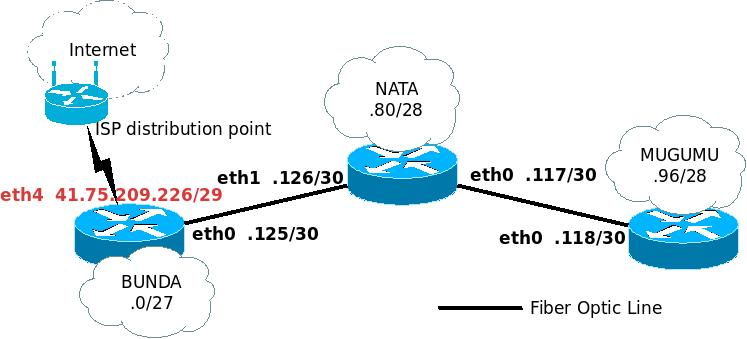
\includegraphics[width=0.8\textwidth]{sbn_all.jpeg}
\caption{An Overview of SBN}
\label{sbn_all}
\end{figure}
The router currently in use is Supermicro X7SPA based system with integrated power supply unit. More of system design is discussed in Section \ref{sysdesign}. The network is then distributed to end users through terrestrial wireless devices. 

\subsection{WiBACK Network}
WiBACK is used to extend Bunda network to the west. WiBACK is essencially relay agent based on MPLS traffic forwarding. It is easy and fast to deploy and features QoS-provisioning, auto-configuration, self-management and self-healing. In SBN context, WiBACK network relies on 802.11 standards and operates in 5GHz domain.

The initial plan was to achieve a topology shown in Figure \ref{wibacknetwork}.
\begin{figure}[htbp]
\centering
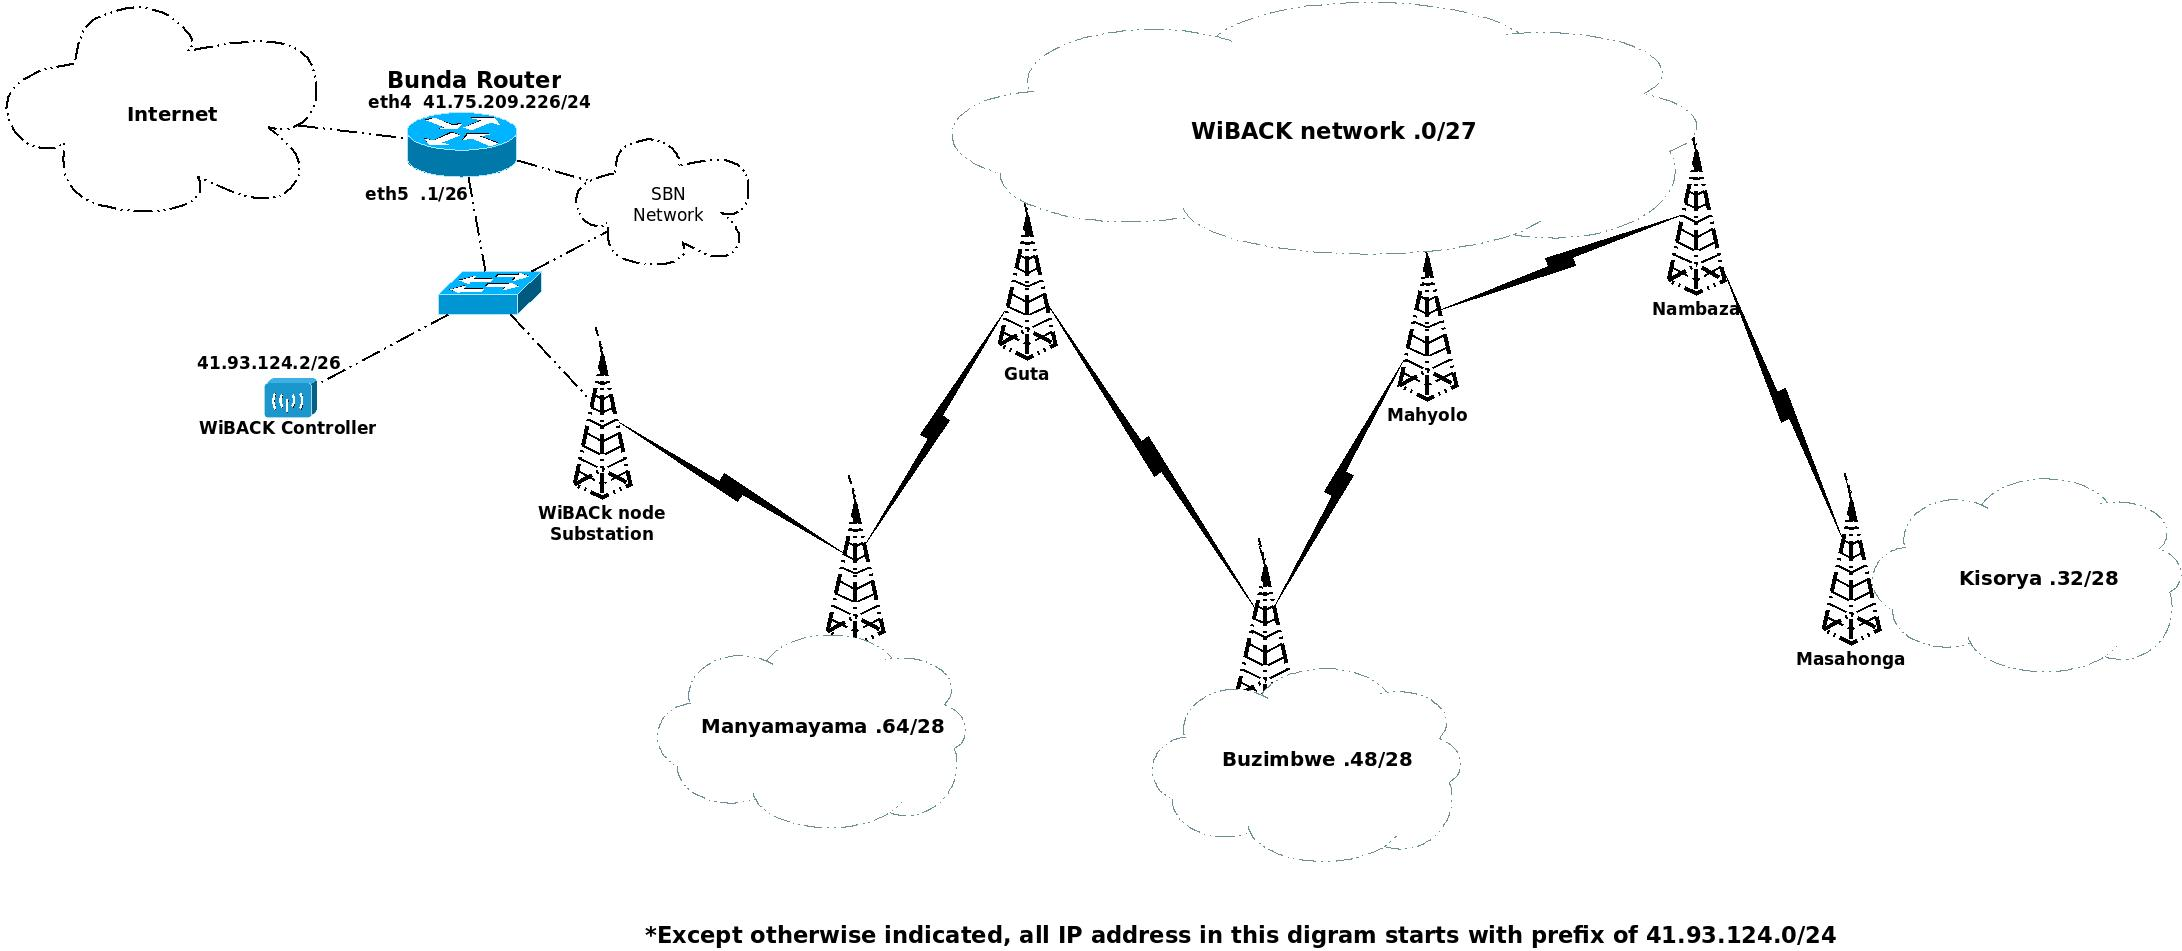
\includegraphics[width=\textwidth]{wibacknetwork.jpeg}
\caption{The initial plan of WiBACK network}
\label{wibacknetwork}
\end{figure}

\subsection{IP Allocation}
IP allocation is listed in Table \ref{ip}. A visualization using Hilbert Curve can be found in Appendix X.
%TODO hilbert curve appendix
\begin{table}[htbp]
\centering
\begin{tabular}{lll}
 \hline
 Domain & IP & Remarks \\
 \hline
 Administration & 0/29 & Administration \\		
 \hline
 WiBACK & 0/27 & Reserved for other WiBACK network\\
 & 32/28 & Kisorya (AIRC) network \\
 & 48/28 & Buzimbwe (Kibara network) \\
 & 64/28 & Manyamayama \\
 \hline
 Serengeti Fiber & 80/28 & Nata \\
 Network & 96/28 & Mugumu \\
 & 80/28 & Nata \\
 & 116/30 & Nata -- Mugumu router \\
 & 124/30 & Bunda -- Nata router \\
 \hline 
 Odroid Testing & 144/28 & Odroid Network Testing (Internal Links) \\
 \hline 
 Tunnels & 128/28 & Tunnels \\
 \hline
\end{tabular}
\caption{IP allocation of SBN}
\label{ip}
\end{table}